\documentclass[12pt]{article}
\usepackage{amsmath,amssymb,bookmark,graphicx,parskip,custom}
\usepackage[margin=.8in]{geometry}
\allowdisplaybreaks
\hypersetup{colorlinks,
    citecolor=black,
    filecolor=black,
    linkcolor=black,
    urlcolor=black
}
\setcounter{secnumdepth}{5}

\begin{document}

\title{SCI 238 --- Introduction to Astronomy}
\author{Kevin James, Eric Pemberton, Lara Janecka, Nik Klassen, Tyler Babaran}
\date{\vspace{-2ex}Winter 2015}
\maketitle\HRule

\tableofcontents
\newpage


\input{chapters/chapter1.tex}
\input{chapters/chapter2.tex}
\input{chapters/chapter3.tex}
\input{chapters/chapter4.tex}
\input{chapters/chapter5.tex}
\input{chapters/chapter6.tex}
\section{Chapter 10 -- Our Star}
\subsection{A Closer Look at the Sun}
\subsubsection{History}
Our first views of the sun were that it was a ball of fire. In the $19^{th}$ century we had found the Sun's radius and distance and found that its energy could not have come from burning fuels or other chemical processes.

The first real idea was that the Sun generates energy by slowly contracting in size through \textbf{gravitational contraction}. Gravitational potential energy is converted into thermal energy as mass moves inward. This would keep the inside of the Sun hot. The amount of contraction required would be small enough to go unnoticed until the $19^{th}$ century. This theory shows that the Sun could continue contracting for 25 million years. The problem: geologists had already calculated the earth's age as much higher than that.

The next idea was based on Einstien's theory of relativity ($E=mc^2$). Calculations showed that the Sun had enough mass to shine for billions of years. This explained where sunlight came from, but not the thermal energy. Eventually in the  1930's the discovery of nuclear fusion was found and we use that to explain where thermal energy comes from.

\subsubsection{Nuclear Fusion}
Nuclear fusion requires very high temperature and density to start. This started in the sun through gravitational contraction. The sun was formed from a collapsing gas cloud. This released gravitational potential energy raisin the core temperature. This continued to happen until sustained nuclear fusion started.

The sun has a fairly steady size and energy today because it has reached equilibrium. \textbf{Gravitaitonal Equilibrium} is the balance between the outward push of hot internal gases trying to escape and the inward push of gravity. This allows the sun to have a steady size. This also means that \textbf{pressure increases with depth} in the sun. \textbf{Energy Balance} is the balance between the rate of fusion and the rate of energy being released from the Sun's core into space.

\subsubsection{Structure}
The sun is essentially a ball of plasma (gas in which atoms are ionized) which moves like a gas, but also reacts to magnetic fields.

Basic Properties:\\
\begin{tabular}{|c|c|}
\hline
Radius (R Sun ) & 696,000 km (about 109 times the radius of Earth)\\
\hline
Mass (M Sun )  & 2 ϫ 10 30 kg (about 300,000 times the mass of Earth)\\
\hline
Luminosity/Power Output (L Sun ) & 3.8 ϫ 10 26 watts\\
\hline
Composition (by percentage of mass) & 70\% hydrogen, 28\% helium,2\% heavier elements\\
\hline
Rotation rate & 25 days (equator) to 30 days (poles)\\
\hline
Surface temperature & 5800 K (average); 4000 K(sunspots)\\
\hline
Core temperature & 15 million K\\
\hline
\end{tabular}

Layers (outside in):
\begin{itemize}
\item Solar wind
\item Corona
\item Chromosphere
\item Photosphere
\item Convection zone
\item Radiation zone
\item Core
\end{itemize}
\textbf{Solar Winds} is a stream of charged particles blown outward from the Sun. These help shape the magnetospheres of planets and the tails of comets.

\textbf{Corona} is suprisingly hot (1 million K) and emits the most X-ray radiation, the density is very low

\textbf{Chromosphere} is much cooler here (10,000 K), radiates UV radiation

\textbf{Photosphere} temperature is 6,000K, surface churns like boiling water, home of sunspots and intense magnetic fields

\textbf{Convection Zone} region of hot gas rising and cool gas sinking caused by energy from the core rising to the surface (called convection, duh)

\textbf{Radiation Zone} less turbulent than the convection zone, energy moves outwards as photons instead of hot gas, temperature rises to 10 million K, shit ton of X-ray radiation

\textbf{Core} where nuclear fusion is making energy, temperature 15 million K, density 100 that of water, pressure 200 billion times earth's surface, energy takes hundreds of thousands of years to get to the surface

\subsection{Nuclear Fusion in the Sun}
Note nuclear fusion (the Sun) $\not =$ nuclear fision (nuclear reactor).

Within the Sun's core there is a soup of hot fas funn of psitively charged atom nuclei flying about. When these collide (most of the time electormagnetic forces deflect them) they stick together to form a heavier nucleus. This is caused by \textbf{strong force} (binds protons and neutrons together) overriding the electromagnetic deflection force. It's only strong enough to do this at very small distances which happens due to the high speed of the particles (which is in turn caused by the high temperature which is caused by the high pressure which is caused by high gravitational force which is caused by large mass).

This is explained by the \textbf{Ideal Gas Law} \[ P = nkT \] where P is the pressure, n is number density (particles per volume), T is temperature, and k is \textbf{Boltzmann constant} $=1.38 \times 10^{-23}$ joule/K

\subsubsection{Proton-Proton Chain}
Most hydrogen comes in the form of a single proton, but we need to fuse it into a helium atom which is two protons and two neutrons. So what we have to do is fuse four hydrogen atoms into one helium atom. This is through a sequence of events called the \textbf{proton-proton chain}.
\begin{enumerate}
\item Two protons fuse to make a deuterium nucleus (1 proton and 1 neutron). This step occurs twice
\item The deuterium nucleus and a proton fuse to make a nucleus of helium-3 (2 protons, 1 neutron). This step occurs twice
\item Two helium-3 nuclei fuse to form helium-4 (2 protons, 2 neutrons), releasing two excess protons in the process.
\end{enumerate}
In total four protons collide to make a helium atom, two positrons, and two neutrinos.

\subsubsection{Solar Thermostat}
Life on earth relies on the Sun's steady fusion rate. If we were to increase the core's temperature slightly, this would cause an increase in fusion rate. The increased fusion rate would make more energy, but energy moves very slowly through the sun so it would get bottled up in the core. This would increase the core pressure to exceed the balancing force of gravity so the core would expand and cool. Cooling lowers the fusion rate and equilibrium is reached again.

\includegraphics[width=\textwidth]{solarThermostat}

\subsubsection{Path of Energy Through the Sun}
Energy starts as photons in the Sun's core. They zigzag at the speed of light so it takes them a while to get out. In the dense interior a photon can only ravel a fraction of a millimeter before it collides with electron and gets deflected in a new direction causing its zigzag path. Eventually it makes its way through the core and radiation zone into the convection zone where the temperature drops to 2 million K and the photon is absorved into cooler solar plasma. This creates the convection that happens in the convection zone. Eventually it rises to the top and enters the photosphere. Here the density is low enough that photons can escape into space as sunlight.

How do we know about the interior of a star:
\begin{itemize}
\item Mathematical models: based on laws of physics and observed properties
\item Solar Vibrations: the Sun's surface vibrates like with earthquakes which we can see in Doppler Shifts.
\item Solar Neutrinos: these are formed during nuclear fusion, these can pass through almost anything without reacting (including the Sun's layers), so we can see whats going on right now (well, 8 minutes ago)
\begin{itemize}
\item these fuckers are hard to catch, need detectors deep in mines
\item initially we only caught a third of what we expected (solar neutrino problem) due to neutrinos changing properties during their journey (electron neutrino, muon neutrino, or tau neutrino)
\end{itemize}
\end{itemize}

\subsection{The Sun-Earth Connection}
\subsubsection{Sunspots and Magnetic Fields}
\textbf{Sunspots} are dark spots on the sun where things are cooler. They are formed when magnetic fields keep hot gas from entering a section of the photosphere. Magnetic fields can alter the energy levels of atoms (Zeeman effect), mucking with their spectral lines. The particles in solar plasma move along magnetic lines (usually spiraling along them).

Sunspots form where magnetic fields extend from the Sun's interior. The magnetic lines there are strong enough to suppress convection making the spot cool. They usually last a few weeks until their magnetic fields weaken. Sunspots tend to appear in pairs connected by a magnetic loop. Gas getting trapped in these loops makes \textbf{solar prominences}.

\subsubsection{Solar Storms}
These are sudden changes in the Sun's magnetic fields. The most dramatic example is \textbf{solar flares} which send bursts of X rays and fast moving particles into space. Flares tend to happen near sunspots. The current theory is that solar flares are caused when magnetic fields become so twisted they cannot bear the tension and snap into a better shape.

\subsubsection{Heating the Chromosphere and Corona}
Some weird shit goes down on the sun where its atmosphere gets hotter the farther you go out. The current theory is that magnetic fields carry energy upward to heat the chromosphere and corona.

The churning that happens in the convection zone probably shakes with tightly wound magnetic lines which carry this energy into the atmosphere and deposit it as heat.

Its very hard to investigate this because the solar atmosphere is not dense enough to see at that point (except during an eclipse). We can watch them through X-rays and UV rays.

In X-ray images of the chronosphere:
\begin{itemize}
\item bright spots is where hot gas is trapped below a sunspot where magnetic lines loop back to the Sun
\item dull spots (\textbf{coronal holes}) are under magnetic lines that escape into space
\item the stuff blown out by flares are huge bubbles called \textbf{coronal mass ejections}
\begin{itemize}
\item have strong magnetic fields
\item causes auroras
\item fuck with satellites
\end{itemize}
\end{itemize}

\subsubsection{Solar Cycles}
Sunspots have a 11 year cycle. The solar maximum has most sunspots and solar minimum has fewest. At each solar maximum the Sun's magnetic fields start to flip. This is because all magnetic lines connecting pairs of sunspots point the same direction. This means that magnetic fields have a 22 year cycle.

\section{Chapter 11 -- Surveying the Stars}
\subsection{Properties of Stars}
\subsubsection{Luminosity}
The \textbf{apparent brightness} of a star is how bright it appears to us, or the amount of power reaching us per unit area (units are watts per square meter). The \textbf{luminosity} of a start is is the total power that the star emits (units are watts). Apparent brightness follows a inverse square law to distance.
\begin{align*}
    \text{apparent brightness} = \frac{\text{luminosity}}{4\pi \times (\text{distance})^2}
\end{align*}

The most direct way to measure a star's distance it through measuring its stellar paralax. This is found by comparing a star's shift against its background over 6 months. We calculate its \textbf{paralax angle} \[ d = \frac{1}{p} \]
Where d is the distance to that star in light years and p is the paralax angle (Note: 1 arcsecond $\rightarrow$ 3.26 lightyears = 1 parsec)

We tend to measure luminosities as orders of magnitude of our sun's luminosity, called \textbf{apparent magnitude} instead of apparent brightness and \textbf{absolute magnitude} instead of luminosity. For every 5 magnitudes we have a brightness factor of 100. So a magnitude 1 star is 100 times brighter than a magnitude 6 star. We define the absolute magnitude as the apparent magnitude if owould have itf it were at a distance of 10 parsecs.

\subsubsection{Temperature}
The temperature of a star usually means its surface temperature since its the easiest to measure. A star's temperature is easier to measure than luminosity since it does not vary with distance. We can measure a star's temperature with reasonable accuracy by measuring its color. This is done by comparing its apparent brightness in two different colors of light (usually blue and red).

We run into problems when interstellar dust interferes with the color of a star so astronomers use a star's spectral lines instead. Stars showing spectral lines of ionized elements are fairly hot because it takes high temperature to ionize atoms. In contrast, stars displying spectral lines of molecules are relatively cool. Stars are classified by their \textbf{spectral type} OBAFGK in decreasing order of temperature. These are often divided farther using numbers. For example our sun is a G2 star meaning its hotter than a G3 but cooler than a G1.

\begin{tabular}{|l|l|l|l|l|}
\hline
Type & Example(s) & Temp. & Key Absorption Line Features & Brightest (color) \\
\hline
O & Stars of Orion’s Belt & $>$30k K & Strong ionized He, weak H & $>$97 nm (ultraviolet) \\
\hline
B & Rigel & 30k-10k K & Strong neutral He, some H & 97-290 nm (ultraviolet) \\
\hline
A & Sirius & 10k-7.5k K & Very strong H & 290-390 nm (violet) \\
\hline
F & Polaris & 7.5k-6k K & Some H, some ionized Ca & 390-480 nm (blue) \\
\hline
G & Sun, Alpha Cent. A & 6k-5k K & Weak H, strong ionized Ca & 480-580 nm(yellow) \\
\hline
K & Arcturus & 5k-3.5k K & some metals, some molecules & 580-830 nm (red) \\
\hline
M & Betelgeuse, Prox. Cent. & $<$3.5k K & Strong molecules & $>$ 830 nm (infrared) \\
\hline
\end{tabular}

\textbf{History of Spectral Types}
Spectral types were made at Harvard College by Edward Pickering's computers (women who'd studied physics or astronomy). The first was Williamina Flemming who classified A-O by the descending strength of hydrogen lines. Annie Jump Cannon modified this existing classification by reordering and removing classes until the OBAFGKM that is used today was left. Finally Cecilia Payne-Gaposchkin discovered that stars were all made of the same material and the lines reflected ionization levels which indicated surface temperature.

\subsection{Mass}
Measuring mass is very difficult and we can only really do it on binary star systems. We do this by applying Newton's version of Kepler's third law

Binary star types:
\begin{itemize}
\item \textbf{visual binary: } we can see each star distinctly, sometimes one star is too dim to see but we can observe the shift of the visible star
\item \textbf{eclipsing: }  a pair of stars that orbit in a plain of our line of sight, we rotate between seeing the combined light of both stars (no eclipse) and only the light of one star (full eclipse)
\item \textbf{spectroscopic: } we need to use Doppler shifts to detect its nature
\end{itemize}

\subsection{Patterns Among Stars}
These are ways of charting stars, the x-axis is the surface temperature (OBAFGKM) and the vertical axis is luminosity ($L_{sun}$) on a logarithmic scale. We can also infer the star's radius from the chart because a star's luminosity is based on its surface temperature and radius.
\begin{align*}
L &= 4\pi r^2 \times \sigma T^4 \\
\sigma &= 5.7 \times 10^{-8} W/(m^2 \times \text{Kelvin}^4)
\end{align*}
Where L is luminosity, r is radius, $\sigma$ is amount of thermal radiation emmited per unit area constant, and T is the star's temperature. This means that the radius of a star increases along a diagonal from lower left to upper right.

Stars cluster on the H-R diagram:
\begin{itemize}
\item \textbf{main sequence: }streak running from upper left to lower right
\item \textbf{supergiants: }upper right
\item \textbf{giants: }between supergiants and main sequence
\item \textbf{white dwarfs: }lower left
\end{itemize}

Like with spectral classes, astronomers assign luminosity classes describing the region of the H-R diagram that a star falls in. I is for super giants, III is for giants and V is for main sequence. II and IV are for those that fall inbetween. White dwarfs fall outside the classification and are called wd. Stars with higher luminosity have larger radii as well.

We combine spectral type and luminosity class together to identify stars.

\subsection{Main Sequence}
Main sequence stars are the majority of stars that we observe and because of that we have found more patterns within them. Mass increases as we go up the strip of main sequence stars on the H-R Diagram. We also see that low mass stars are much more common than high mass stars. Mass is the most important attribute of hydrogen fusing stars because it determines the balance point at which energy released by fusion equals the energy lost from the star's surface. This is what allows for the wide range of luminosities. Luminosity is very sensitive to mass (example a star 10 times as massive as the sun is 10000 times as luminous).

A luminous star must be very hot or very large. But a very small mass change is required to greatly increase the luminosity of a star, so their surface temperature must be much higher to account for this large increase in luminosity. This fits the H-R Diagram pattern of temperature increasing with luminosity. We can use the mass-luminosity-temperature relationship to estimate a star's mass just by knowing its spectral type.

A star is born with a set amount of hydrogen fuel, the amount of time that it can burn this fuel for is the star's \textbf{main sequence lifetime}. Lifetime is inversely proportional to the mass of the star. This is because as mass increases luminosity increases exponentially, so stars with higher masses may have more fuel but they burn it waaaay faster.

\subsection{Giants, Supergiants, and White Dwarfs}
\subsubsection{Giants and Supergiants}
These are much cooler but more luminous than the sun which tells us that they are huge. These stars have almost exhausted their hydrogen fuel supply and are trying not to collapse under their own weight. They do this by releasing fusion energy at a high rate which explains their high luminosity, and the need to radiate all this energy expands them to enormous size.

\subsubsection{White Dwarfs}
This is what happens when a giant runs out of fuel completely. The star ejects all of its outer layers and is left only with a dormant core. They are hot because they are still the core of a star, but dim because they have no way to radiate their energy.

\subsection{Star Clusters}
Stars are born from giant clouds and many stars can be born from the same cloud, so they tend to cluster.
\begin{itemize}
\item all stars in a cluster are about the same distance from earth
\item all stars in a cluster are about the same age
\end{itemize}

\subsubsection{Types of clusters}
\begin{itemize}
\item \textbf{open cluster: }found in disk of galaxy, young stars, up to several thousand stars, about 30 light years across
\item \textbf{globular cluster: }found in halo of galaxy: oldest stars, more than a million stars, 60-150 light years across
\end{itemize}

\subsubsection{Age of a Cluster}
We plot a cluster's stars on the H-R Diagram, and this tells us its age. For instance the Pleides open cluster has no stars of the O spectral class. This means that Pleidas is old enough that its O stars have finished their hydrogen fission and `died'. We call the point at which a cluster's main sequence diverges from the standard main sequence the \textbf{main sequence turnoff}. The age of the cluster is equal to the lifetime of stars at its main-sequence turnoff point (at its most massive star).

\input{chapters/chapter14.tex}
\input{chapters/chapter15.tex}
\input{chapters/chapter18.tex}

\section{Assignments}
\input{assignments/assignments1-5.tex}
\section{Assignment 12}

\subsection{Dark matter}

\begin{itemize}
    \item Effects the orbits of stars and gas, causing faster motion than we can account for
    \item Stellar masses only account for most of the total mass close to the center of a galaxy
    \item total mass - luminous mass - mass of hot gas = dark matter
    \item Two main options
    \begin{itemize}
        \item Ordinary - made of protons, neutrons, electrons.  Simply can't be detected
        \item Extraordinary - weakly interacting massive particles (WIMPs).  Mysterious netruino-like particles.  This is the best bet
    \end{itemize}
    \item There isn't enough ordinary matter to explain ordinary dark matter
    \item Evidence:
    \begin{itemize}
        \item Masses measured for galaxy motions
        \item Temperature of hot gas (can be used to determine mass of galaxy)
        \item Gravitational lensing
    \end{itemize}
    \item WIMPs can't collapse because they don't radiate away their energy.  They helped protogalactic clouds collapse without collapsing themselves
    \item Dark matter lumps the universe together; accounting for expansion, galaxies are being drawn together into chains and sheet.
\end{itemize}

A rotation curve is a plot showing orbital speed versus distance form the center.
\begin{itemize}
    \item Rigid disk = proportional
    \item Solar system = decreasing exponential
    \item spiral galaxy = increases as you move away from the center then levels off
\end{itemize}

Rotation curves show us that instead of velocity decreasing as you move away from the center of a galaxy, it increases, or remains constant.  Both indicate that more mass is contained within the orbit than we would expect

\item $v = \sqrt{\frac{M_r * G}{r}}$
\begin{itemize}
    \item $M_r$ = encircled mass
    \item $r$ = radius of sphere containing the mass
\end{itemize}

Definitions

WIMPS: subatomic particles that have more mass than neutrinos but do not interact with light
Baryonic matter: Matter made from ordinary atoms
Gravitational lensing: The effect made when a massive object distorts the light coming from objects behind it

\subsection{Dark Energy}

Galaxies are expanding at an ever-increasing rate.  This is impossible if gravity is the only force involved as it would cause the speed of galaxies to decrease.

The energy causing this repulsion is called dark energy.

Critical density: The average density of the universe such that:
density $<$ critical density $\Rightarrow$ the universe expands at an ever decreasing rate, but never stops.
density $>$ critical density $\Rightarrow$ the universe stops expanding the collapses.

If a critical universe has an average density of one, our universe is $\approx 0.3$.  So it should be coasting.

Dark energy makes it so that instead of the rate of expansion slowing, it is actually increasing.  This also gives us the \textbf{oldest} model of the universe.

The is the age of the universe that would occur from each situation is ordered from youngest to oldest.  Youngest = recollapsing, critical, coastingg, accelerating = oldest.

Dark energy fills the void needed to explain why CMB says the universe is flat.

\subsection{Gravitational Lensing}

The object being lensed is more widely separated when the object doing the lensing is
\begin{enumerate}[a)]
    \item more massive
    \item closer to the Earth
\end{enumerate}

\subsection{Eras of the Universe}

\begin{tabular}{c|c|c|c}
    Era name & description & ended after & temperature at end (K) \\
    Planck & all 4 forces operated as one & $10^{-43} s$ & $10^{32}$ \\
    GUT & strong electroweak forces unit as GUT force & $10^{-38} s$ & $10^{29}$ \\
    Electroweak & 3 forces operated: gravity, strong, electroweak & $10^{-10} s$ & $10^{15}$ \\
    Particle & Protons, neutrons both common & $10^{-3} s$ & $10^{12}$ \\
    Nucleosynthesis & fusion create helium nuclei & 5 minutes & $10^{9}$ \\
    Nuclei & H, He nuclei and electrons existed, but no neutral atoms & 380,000 years & 3000 \\
    Atoms & Neutral atoms existed, but not stars & & \\
    Galaxies & Stars and galaxies common & &
\end{enumerate}

The Planck era was the hottest era, the galaxy era the coolest.

\subsection{Cosmic microwave background}

In the era of nuclei electrons were free, and photons bounced among them.  Once the age of nuclei ended the electrons were captured, and finally able to travel freely.  The temperature of the universe was about 3000 K at this point and was the peak wavelength.  Since then the wavelength has been decreasing linearly with the expansion of the universe.

Wavelength of CMB $\propto$ relative expansion of the universe.

The CMB has a perfect thermal radiation spectrum.  Since it was originally all contained in a small area, where temperature and density could equalize.

Current temperature of the CMB is approximately 2.73 K.


\section{Definitions}
\input{misc/definitions.tex}

\section{Formulae and Values}
Our solar system was formed 4.5 billion years ago, when about $2\%$ of the galaxy's original Hydrogen and Helium had been converted to heavier elements. Thus the cloud which formed our galaxy was roughly $98\%$ Hydrogen and Helium. The $2\%$ of other materials form the core of the rocky planets in our systems, ie. the Earth.

The {\bf Andromeda galaxy} is roughly 2.5 million light-years away and about $100,000$ light-years in diameter. {\bf Sirius}, the brightest star visible in the night sky, is 8 light-years away. {\bf Alpha Centauri}, the closest star system to our own (a three star system), is 4.4 light-years away.

\begin{itemize}
\item $E_k = \frac{1}{2}mv^2$
\item $v = \lambda f$
\item $\text{Energy} = h f = \frac{hc}{\lambda}$
\item $v_\text{radial} = \frac{\Delta \lambda}{\lambda}\ c$
\item $F = G\frac{m_1 m_2}{r^2}$
\item $p^2 = \frac{4\pi^2}{(M_1 + M_2) * G}\ a^3$ (in our solar system $\text{years}^2 = \text{A.U.}^3$)
\item $L = 4\pi^2R^2 \sigma_{SB} T^4$
\item Angular separation (rad) $= \frac{\text{semi-major axis (AU)}}{\text{distance parsecs}}$
\item $r_\text{planet} \approx r_\text{star} * \sqrt{\text{fraction of light blocked}}$
\item Eccentricity of an ellipse: $e = \frac{f}{a}$ where f is the distance from the center to a focus
\item $\text{momentum} = \text{mass} * \text{velocity}$
\item $\text{SA}_\text{sphere} = 4 \pi r^2$
\item $\lambda_\text{peak} T = 2.898 * 10^{-3} m \cdot K$
\item Time dilation: $t' = t * \sqrt{1 - \left( \frac{v}{c} \right)^2}$
\item Length contraction: $l' = l * \sqrt{1 - \left( \frac{v}{c} \right)^2}$
\item Mass increase: $m' = \dfrac{m}{\sqrt{1 - \left( \frac{v}{c} \right)^2}}$
\item Angular size, physical size, and distance are related as $\frac{l_{angular}}{360} = \frac{l_{physical}}{2\pi d}$
\item $v = \sqrt{\frac{M_r * G}{r}}$
\begin{itemize}
    \item $M_r$ = encircled mass
    \item $r$ = radius of sphere containing the mass
\end{itemize}
\end{itemize}


\section{Data}
\begin{description}
\item[Speed of light] $2.998 * 10^8 m/s$
\item[Light year] $9.461 * 10^{15}$ m = 63 241 AU
\item[Parsec] 1 pc = $3.08567758 * 10^{16} m$
\item[Observable Universe Boundary] $~14 * 10^9$ ly
\item[Average Earth-Moon distance] 385 000 km
\item[Average Earth-Sun distance (1 AU)] $1.4959 * 10^{11}$ m
\item[Diameter of the Sun] $1.391 * 10^6$ km
\item[Planck's constant (h)] $6.626 * 10^{-34} J \cdot s = 4.136 * 10^{-15} eV \cdot s$
\item[Stefan-Boltzmann constant] $5.67 * 10^{-8} \frac{W}{m^2 K^4}$
\item[Gravitational constant] $6.673 * 10^{-11} N \cdot (m/kg)^2$
\item[Hubble's Constant] $\approx 70 km/s/Mpc$
\end{description}

\begin{center}
\scalebox{0.8}{
    \begin{tabular}{|p{2.5cm}|*{10}{c|}}
    \hline
    & Mercury & Venus & Earth & Moon & Mars & Jupiter & Saturn & Uranus & Neptune & Pluto \\
    \hline
    Mass ($10^{24}$ kg) &  0.330 &  4.87 &  5.97 &  0.073 &  0.642 &  1898 &  568 &  86.8 &  102 &  0.0131 \\ \hline
    Diameter (km) &  4879 &  12,104 &  12,756 &  3475 &  6792 &  142,984 &  120,536 &  51,118 &  49,528 &  2390 \\ \hline
    Density ($kg/m^3$) &  5427 &  5243 &  5514 &  3340 &  3933 &  1326 &  687 &  1271 &  1638 &  1830 \\ \hline
    Gravity ($m/s^2$) &  3.7 &  8.9 &  9.8 &  1.6 &  3.7 &  23.1 &  9.0 &  8.7 &  11.0 &  0.6 \\ \hline
    Escape Velocity (km/s) &  4.3 &  10.4 &  11.2 &  2.4 &  5.0 &  59.5 &  35.5 &  21.3 &  23.5 &  1.1 \\ \hline
    Rotation Period (hours) &  1407.6 &  -5832.5 &  23.9 &  655.7 &  24.6 &  9.9 &  10.7 &  -17.2 &  16.1 &  -153.3 \\ \hline
    Length of Day (hours) &  4222.6 &  2802.0 &  24.0 &  708.7 &  24.7 &  9.9 &  10.7 &  17.2 &  16.1 &  153.3 \\ \hline
    Distance from Sun ($10^6$ km) &  57.9 &  108.2 &  149.6 &  0.384* &  227.9 &  778.6 &  1433.5 &  2872.5 &  4495.1 &  5870.0 \\ \hline
    Perihelion ($10^6$ km) &  46.0 &  107.5 &  147.1 &  0.363* &  206.6 &  740.5 &  1352.6 &  2741.3 &  4444.5 &  4435.0 \\ \hline
    Aphelion ($10^6$ km) &  69.8 &  108.9 &  152.1 &  0.406* &  249.2 &  816.6 &  1514.5 &  3003.6 &  4545.7 &  7304.3 \\ \hline
    Orbital Period (days) &  88.0 &  224.7 &  365.2 &  27.3 &  687.0 &  4331 &  10,747 &  30,589 &  59,800 &  90,588 \\ \hline
    Orbital Velocity (km/s) &  47.4 &  35.0 &  29.8 &  1.0 &  24.1 &  13.1 &  9.7 &  6.8 &  5.4 &  4.7 \\ \hline
    Orbital Inclination (degrees) &  7.0 &  3.4 &  0.0 &  5.1 &  1.9 &  1.3 &  2.5 &  0.8 &  1.8 &  17.2 \\ \hline
    Orbital Eccentricity &  0.205 &  0.007 &  0.017 &  0.055 &  0.094 &  0.049 &  0.057 &  0.046 &  0.011 &  0.244 \\ \hline
    Axial Tilt (degrees) &  0.01 &  177.4 &  23.4 &  6.7 &  25.2 &  3.1 &  26.7 &  97.8 &  28.3 &  122.5 \\ \hline
    Mean Temperature (C) &  167 &  464** &  15 &  -20 &  -65 &  -110 &  -140 &  -195 &  -200 &  -225 \\ \hline
    Surface Pressure (bars) &  0 &  92 &  1 &  0 &  0.01 &  Unknown &  Unknown &  Unknown &  Unknown &  0 \\ \hline
    Number of Moons &  0 &  0 &  1 &  0 &  2 &  67 &  62 &  27 &  14 &  5 \\ \hline
    Ring System? &  No &  No &  No &  No &  No &  Yes &  Yes &  Yes &  Yes &  No \\ \hline
    Global Magnetic Field? &  Yes &  No &  Yes &  No &  No &  Yes &  Yes &  Yes &  Yes &  Unknown \\ \hline
    \end{tabular}
}
\end{center}
{\footnotesize * From the Earth}\\
{\footnotesize ** Due to intense greenhouse effect of thick atmosphere}\\

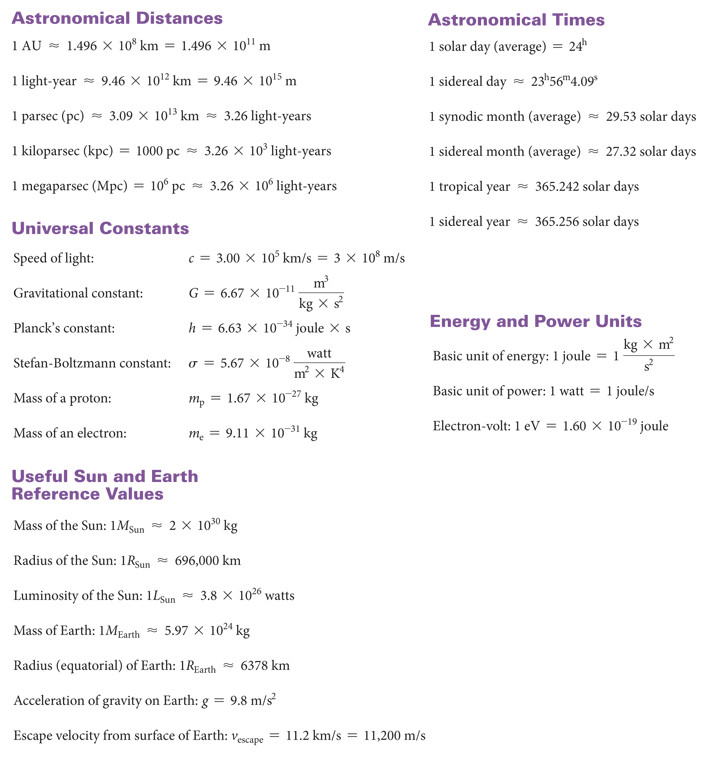
\includegraphics[scale=0.7]{constants}


\section{Lecture Slides}
\input{slides/scale.tex}
\input{slides/discovery.tex}
\input{slides/science.tex}
\input{slides/making_sense.tex}
\input{slides/light.tex}
\input{slides/telescopes.tex}
\input{slides/system.tex}
\input{slides/distant.tex}
\input{slides/life.tex}
\section{Chapter S3: Space and Time}

\subsection{Special Relativity}

Einstein's Theories of Relativity:
\begin{itemize}
\item Special Relativity: usual ideas of space and time change as we approach the speed of light ($E = mc^2$)
\begin{itemize}
\item no object can travel faster than light
\item observing a object near the speed of light:
\begin{itemize}
\item time slows down
\item length contracts in direction of motion
\item mass increases
\end{itemize}
\item simultaneousness changes based on your frame of reference
\end{itemize}
\end{itemize}

Postulates of special relativity:
\begin{itemize}
\item laws of nature are the same for everyone
\item speed of light is the same for everyone
\end{itemize}

Time Dilation: \[ t_1 = t_0\sqrt{1-\bigg(\frac{v^2}{c^2}\bigg)} \]
Length Contraction: \[ l_1 = l_0\sqrt{1-\bigg(\frac{v^2}{c^2}\bigg)} \]
Mass Increase: \[ m_1 = \frac{m_0}{\sqrt{1-\bigg(\frac{v^2}{c^2}\bigg)}} \]

Since no information can be transfered faster than the speed of light objects traveling near the speed of light will perceived information at different rates since the information is moving much more slowly relative to their speed.

\subsubsection{Tests for Relativity}
Michelson-Morley experiment found evidence for the absoluteness of the speed of light in 18887.

Time dilation occurs often to subatomic particles in accelerators.

Time dilation discovered with airplanes and very precise clocks.

$E = mc^2$ verified by measurements taken of the sun.

If the speed of light were not absolute light coming from a car moving towards you would travel at 100km/hr + c and a car moving parallel to you would be see at 100 km/hr so witnessing their collision would look very odd.

\subsection{General Relativity:}

\begin{itemize}
    \item Gravity arises from distortions of spacetime
    \item Time runs slowly in gravitational fields
    \item Rapid changes in the motion of large masses can cause \emph{gravitational waves}
\end{itemize}

\textbf{The equivalence principle:} Being on Earth (gravity = 1g) is exactly equivalent to being in space accelerating at 9.8 $m/s^2$ (1g) feel the exact same.

Motion is relative. Usually how fast your perceive something is based on your velocity compared to it. The exception is light which always is seen at the same speed (called \textbf{absolute relativity})

Worldlines:
\begin{itemize}
    \item x-axis = space
    \item y-axis = time
    \item vertical line = no motion
    \item diagonal line = constant motion
\end{itemize}

What are the effects of a curved geometry for spacetime?
\begin{itemize}
    \item The shortest path between two points is a great circle
    \item Parallel lines eventually converge
    \item Angles in triangles add up to $> 180^\circ$
    \item Circumference of a circle is $< 2\pi r$
\end{itemize}

Saddle-shaped geometry
\begin{itemize}
    \item A piece of a hyperbola is the shortest distance between two points
    \item Parallel lines diverge
    \item Angles in a triangle $< 180^\circ$
    \item Circumference of a circle is $> 2\pi r$
\end{itemize}

According to the equivalence principle if you are floating freely, then your worldline is following the \textbf{straightest possible path} through spacetime.  If you feel weight, then your path is curving.


Curvature of spacetime depends on the size of the object and the mass of the object:  If we change the size of an object without changing its mass, spacetime becomes more curved near its surface (as does the strength of gravity).

In a black hole the curvature forms a ``bottomless pit'' in spacetime.  The point of no return in a black whole is the \textbf{event horizon}, where the escape velocity surpasses the speed of light.

\subsubsection{Gravity and Time}

In an accelerating spaceship, light travels more quickly from front to back than vice versa.  So we say that time is running more quickly in the front of the spaceship.  By the equivalence principle, time runs slower at lower altitudes

\subsubsection{Evidence for general relativity}

\begin{itemize}
    \item Precession of mercury
    \item Gravitational lensing: light bends around very massive objects
    \item Gravitational time dilation
    \item Gravitational waves
    \begin{itemize}
        \item movements of a massive object can produce gravitational waves
        \item we think we have observed this in the orbits of a binary neutron star system (orbit is getting smaller as energy is carried away)
    \end{itemize}
\end{itemize}

\input{slides/stars.tex}

\end{document}
